\documentclass{beamer}
\usepackage[utf8]{inputenc}
\usepackage{url}
\usepackage{amsmath}
\usepackage{amssymb}
\usepackage{graphicx}
\usepackage{color}
\usepackage{amsthm}
\usepackage{amsfonts}
\definecolor{midnight}{RGB}{25,25,112}
\mode<presentation>{
	\usetheme{Singapore}
	\usecolortheme[named=midnight]{structure}
	\setbeamertemplate{navigation symbols}{} % rids of nav bar
	\setbeamertemplate{footline}[frame number] % number slides
}

\title{Hard-margin SVM}
\author{Levent Sagun}
\institute{New York University}
\date{February 11, 2016}

%------------------------------------------------------------

\begin{document}

%------------------------------------------------------------

\frame{\titlepage}

%---------------------------------------------------------

\begin{frame}
\frametitle{Problem setup}

Given a set of linearly separable training data, how can one find a good separator? What do we expect from a good separator? 

\begin{itemize}
    \item<1-> ... that it actually separates the training points
    \item<1-> ... that it generalizes well
\end{itemize}

Let $\{x^i, y^i\}_{i=1}^N \in \mathcal{D} $ be the training data, where $x^i \in \mathbb{R}$ and $y^i$ is either +1 or -1. What does it mean that the data is linearly separable?

\begin{itemize}
    \item<1-> ... that there is a hyperplane that separates the two clusters
    \item<1-> ... that there is possibly \textit{a lot} of such hyperplanes
\end{itemize}

How to choose the best one?

\end{frame}
 
%---------------------------------------------------------

\begin{frame}{Example}
    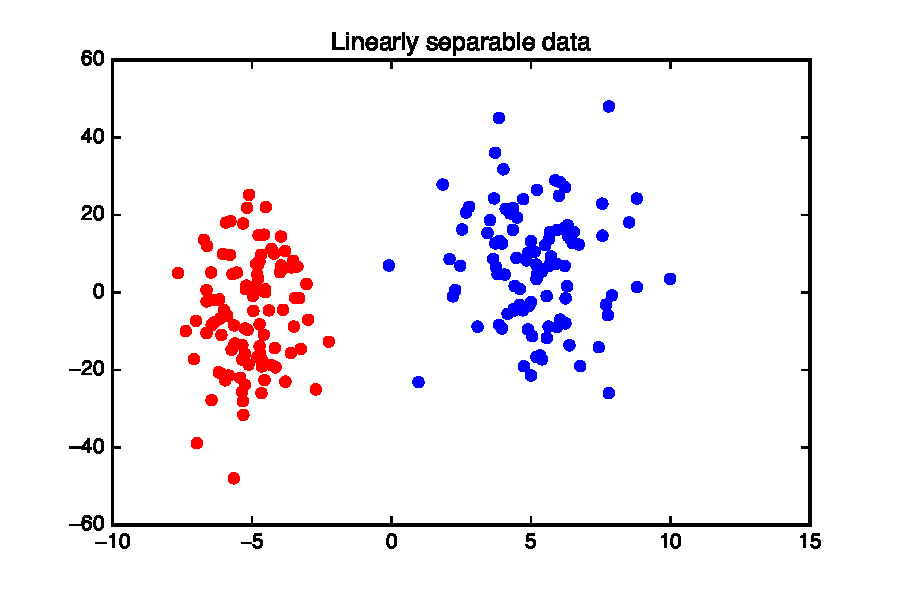
\includegraphics[scale=0.7]{figures/SVM_data.pdf}
\end{frame}

%---------------------------------------------------------

\begin{frame}{Example}
    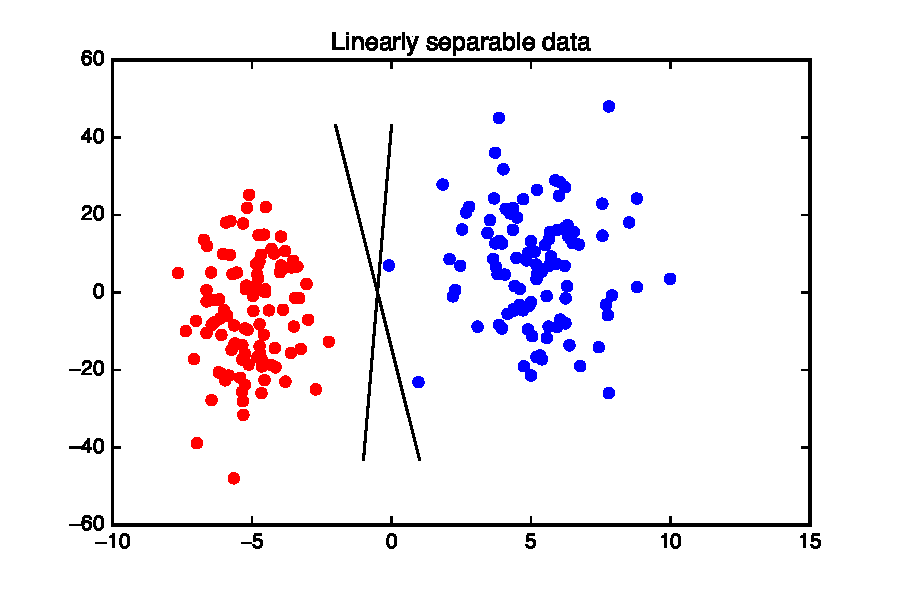
\includegraphics[scale=0.7]{figures/SVM_data_lines.pdf}
\end{frame}

%---------------------------------------------------------

\begin{frame}{Example}
    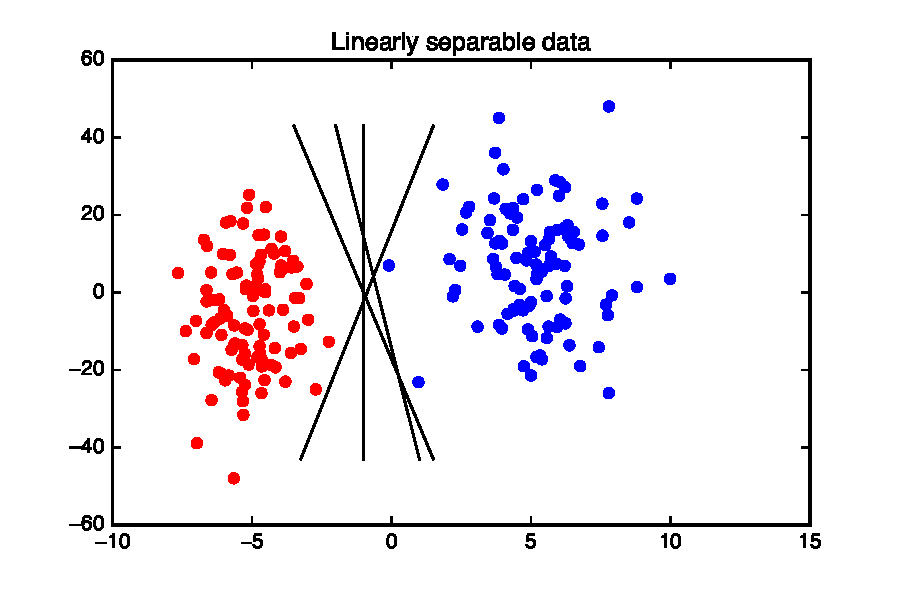
\includegraphics[scale=0.7]{figures/SVM_data_morelines.pdf}
\end{frame}

%---------------------------------------------------------

\begin{frame}{Hyperplane parametrization}

Simplest case of real variables, $y = mx + b$ draws a line with slope $m$ that intersects $y$-axis at the point $b$:

\begin{itemize}
    \item Rewrite the above equation: $(m, -1) \cdot (x, y) + b = 0$
    \item A better notation can be: $(w_1, w_2) \cdot (x_1, x_2) + b = 0$ \item $-w_2/w_1 = m$ captures the connection between the two
\end{itemize}
\pause
Generalize this to higher dimensions, for $w, x \in \mathbb{R}^n$ and $b \in \mathbb{R}$:
\begin{itemize}
    \item $ \ell(x) = w\cdot x + b$ where $\ell(x) = 0$ describes a line.
    \item $w$ is orthogonal to $\ell$ (check $w\cdot v = 0$ for $v$ along $\ell$.)
    \item What should $\ell$ assign to the two clusters?
        \[
        \ell(x) \text{ is } 
        \begin{cases}
        > 0 \text{ if } x \in \text{Blue: $+1$ class} \\
        < 0 \text{ if } x \in \text{Red: $-1$ class}
        \end{cases}
        \]
    \item \textit{Observation:} $y^i\ell(x^i)$ is always positive!
\end{itemize}
    
\end{frame}

%---------------------------------------------------------

\begin{frame}{Distance of a point to a line}

For a point $x \in \mathbb{R}^n$, how far is $x$ to a given line $\ell$?
\begin{itemize}
    \item Denote the distance of a point $x$ to a line $\ell$ by $d(x,\ell)$.
    \item Pick a point on the line, say $x'$, then $d(x,\ell)$ is the projection of $(x-x')$ onto the normal vector $w$ of $\ell$.
\end{itemize}

\begin{columns}
\column{0.52\textwidth}
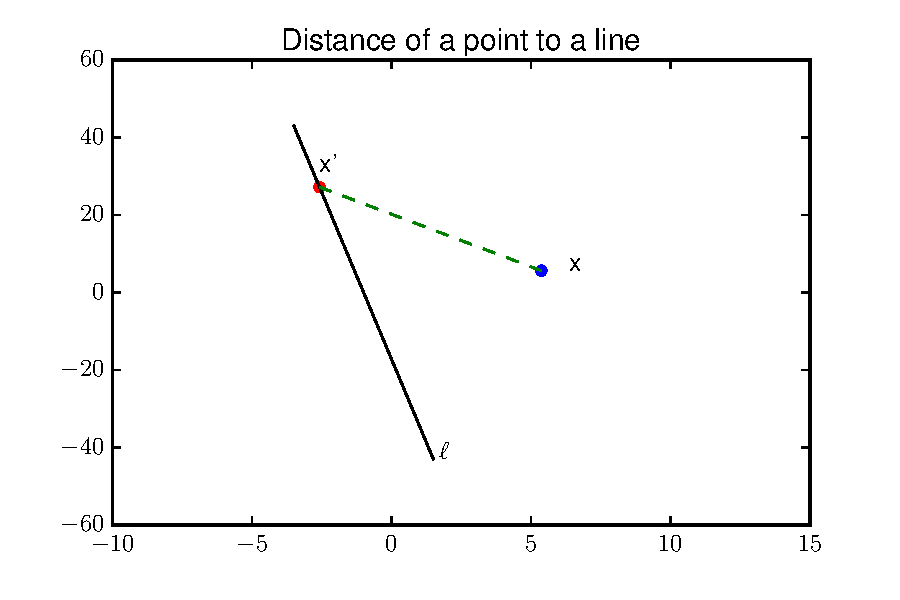
\includegraphics[scale=0.4225]{figures/proj.pdf}

\column{0.6\textwidth}
Crash course on projections:
\begin{itemize}
    \item Linear transformations, $P$, such that $P^2=P$.
    \item Unique decomposition into image and kernel of $P$
    \item Orthogonal projections: $P=P^T$
    \item Vector projection: $P_w(v)=\frac{v\cdot w}{||w||^2}w$
\end{itemize}
\end{columns}
    
\end{frame}

%---------------------------------------------------------

\begin{frame}{Hard-margin SVM}

Given two linearly separable clusters, $\mathcal{C}_1$ and $\mathcal{C}_2$, and a line $\ell$ with $ \ell(x) = w\cdot x + b$ and $||w||=1$, suppose $x^{1,\ell} \in \mathcal{C}_1$ and $x^{2,\ell} \in \mathcal{C}_2$ are the closest points to $\ell$.
\begin{itemize}
    \item For any $i$, $y^i\ell(x^i) \geq \min \{d(x^{1,\ell},\ell), d(x^{2,\ell},\ell)\}> 0 $
    \item \textbf{GOAL:} Maximize the \textit{margin}!%: $\max\{ d(x^{1,\ell},\ell)+d(x^{2,\ell},\ell)\}$
    \item Since data is linearly separable, the maximizer will be on the set where $d(x^{1,\ell},\ell)=d(x^{2,\ell},\ell)$, let's call this $M$.
    
    (note that $M$ depends on data points and the line)
\end{itemize}

\pause
\vspace{0.5cm}
\textbf{Procedure:}
\begin{align}
& \max \{M:b\in\mathbb{R}, w \in\mathbb{R}^n, ||w||=1\} \\
& \text{subject to } y^i(w\cdot x^i + b)\geq M
\end{align}

\end{frame}

%---------------------------------------------------------

%---------------------------------------------------------

\begin{frame}{Equivalent formulation}

For any pair of $(w,b)$ we can calculate $M$ and then considering the new pair $(w',b')=(\frac{w}{M}, \frac{b}{M})$ we get $y^i(\frac{w}{M}\cdot x^i + \frac{b}{M})\geq 1$. Therefore, maximizing $M$ can be rephrased as minimizing $||w'||$.

\vspace{0.5cm}
\textbf{New procedure:}
\begin{align}
& \min \{||w'||:b'\in\mathbb{R}, w' \in\mathbb{R}^n\} \\
& \text{subject to } y^i(w'\cdot x^i + b')\geq 1
\end{align}
\begin{itemize}
    \item Note that: $||w'||=||\frac{w}{M}||=\frac{||w||}{M}=\frac{1}{M}$
    \item This is a convex optimization problem: quadratic criterion, linear inequality constraints.
    \item But, what if the clusters overlap?
\end{itemize}
\end{frame}

%---------------------------------------------------------

\begin{frame}{Overlapping clusters}
    For all data points let $t^i > 0 $ be the slack variables. Let's modify equation (2) to allow each point to have a little more room:
    \[
    \text{subject to } y^i(w\cdot x^i + b)\geq M(1 - t^i) 
    \]
    
    Equivalent formulation ... :
    \[
    \min ||w||, \text{ subject to } y^i(w\cdot x^i + b)\geq 1 - t^i \text{ and } \sum t^i < C
    \]
    
    Equivalent formulation ... :
    \[
    \min \frac{1}{2}||w||^2 + c\sum t^i \\ 
    \text{ subject to } y^i(w\cdot x^i + b)\geq 1 - t^i
    \]
\end{frame}

%---------------------------------------------------------

\begin{frame}{Overlapping clusters}
properties, interpretation, plots...    
\end{frame}

%---------------------------------------------------------

\begin{frame}{Exercises}
\begin{itemize}
    \item \textit{Linear regression;} Minimizing sum of squares of errors in $y=X\beta + \epsilon$:  Find $\beta$ such that $||y-X\beta||=f(\beta)$ is minimized. 
    \item What's the orthogonal projection of $y$ onto the columns of $X$?
    \item What's the connection of the two?
    \item When is $X^TX$ not invertible?
    \item In the overlapping case, what would happen if you modified the constraint by $y^i(w\cdot x^i - b) \geq M - t^i$
\end{itemize}
\end{frame}

%---------------------------------------------------------

\end{document}